\documentclass[a4paper,12pt]{article}

% --- LANGUAGE & FONT ---
\usepackage{vntex}
\usepackage[english]{babel}
\usepackage{amsmath, amssymb}

% --- PAGE & TEXT LAYOUT ---
\usepackage{a4wide}
\usepackage{geometry}
\geometry{a4paper, left=2cm, right=2cm, top=2.5cm, bottom=4.2cm, footskip=12mm}
\usepackage{setspace}
\usepackage{multicol}
\usepackage{enumitem}

% --- GRAPHICS & TABLES ---
\usepackage{graphicx}
\usepackage{epsfig}
\usepackage{svg}
\usepackage{tikz}
\usetikzlibrary{arrows,snakes,backgrounds,positioning,shapes,calc,fit}
\usepackage{booktabs}
\usepackage{multirow}
\usepackage{tabularx}
\usepackage{makecell}
\usepackage{array}
\usepackage[skip=5pt]{caption}
\usepackage{placeins}
\usepackage{float}       % added: the template uses [H]
\usepackage{longtable}   % added: long tables across pages

% --- COLOURS & CODE ---
\usepackage{color}
\usepackage{xcolor}
\usepackage{colortbl}    % added: coloured table rows
\usepackage{minted}
\usepackage{listings}
\usepackage{algorithm}
\usepackage{algpseudocode}
\usepackage[framemethod=tikz]{mdframed}

% --- HEADER & FOOTER ---
\usepackage{fancyhdr}
\usepackage{lastpage}

% --- HYPERREF (always load last) ---
\usepackage{hyperref}
\hypersetup{urlcolor=blue,linkcolor=black,citecolor=black,colorlinks=true}

% ================= COLOURS =================
\setlength{\columnseprule}{1pt}
\def\columnseprulecolor{\color{black}}
\definecolor{p1}{RGB}{52,101,164}
\definecolor{p2}{RGB}{78,154,6}
\definecolor{p3}{RGB}{204,0,0}
\definecolor{p4}{RGB}{117,80,123}
\definecolor{p5}{RGB}{193,125,17}
\definecolor{p6}{RGB}{32,128,128}
\definecolor{p7}{RGB}{90,90,90}
\definecolor{p8}{RGB}{170,60,120}

% ================= HEADER/FOOTER =================
\everymath{\color{blue}}
\setlength{\headheight}{40pt}
\pagestyle{fancy}
\fancyhead{}
\fancyhead[L]{
 \begin{tabular}{rl}
    \begin{picture}(25,15)(0,0)
    \put(0,-8){
\includegraphics[width=8mm, height=8mm]{hcmut.png}}
   \end{picture}&
    \begin{tabular}{l}
        \textbf{\ttfamily Ho Chi Minh City University of Technology - VNU-HCM}\\
        \textbf{\ttfamily Faculty of Computer Science and Engineering}
    \end{tabular}
 \end{tabular}
}
\fancyhead[R]{}
\fancyfoot{}
\fancyfoot[L]{\scriptsize \ttfamily \textcolor{blue}{Builders Buildathon 2026 - P1 Mech Royale \\ Team HCMUT TMT, November 2026}}
\fancyfoot[R]{\scriptsize \ttfamily Page {\thepage}/\pageref{LastPage}}
\renewcommand{\headrulewidth}{0.3pt}
\renewcommand{\footrulewidth}{0.3pt}

\setcounter{secnumdepth}{4}
\setcounter{tocdepth}{3}

% ================= COLOURED BOXES =================
% \partbox{color}{title}{content}: short box, no page break
\newcommand{\partbox}[3]{%
\begin{mdframed}[nobreak=true,linecolor=#1,linewidth=1.2pt,topline=false,rightline=false,bottomline=false,leftmargin=0pt,rightmargin=0pt,innerleftmargin=10pt,backgroundcolor=#1!6]
\textbf{\color{#1}#2}\par\smallskip #3
\end{mdframed}}
% \longbox{color}{title}{content}: long box, may break across pages
\newcommand{\longbox}[3]{%
\begin{mdframed}[linecolor=#1,linewidth=1.2pt,topline=false,rightline=false,bottomline=false,leftmargin=0pt,rightmargin=0pt,innerleftmargin=10pt,backgroundcolor=#1!6]
\textbf{\color{#1}#2}\par\smallskip #3
\end{mdframed}}
% \metabox{color}{workload}{prerequisites}{foundation for}{people}
\newcommand{\metabox}[5]{%
\begin{mdframed}[nobreak=true,linecolor=#1,linewidth=1pt,leftmargin=0pt,rightmargin=0pt,backgroundcolor=#1!15]
\textbf{Workload:} #2\par
\textbf{Prerequisites:} #3\par
\textbf{Foundation for:} #4\par
\textbf{People:} #5
\end{mdframed}}

% ================= HELPER MACROS (added for this report) =================
% \trial{...}: trial-run figure, not an official result
\newcommand{\trial}[1]{\textcolor{p5}{\textbf{[trial run]}~#1}}
% \src{...}: source of a figure
\newcommand{\src}[1]{{\footnotesize\textcolor{p7}{(source: #1)}}}
\newcommand{\fn}[1]{\texttt{\detokenize{#1}}}
\newcolumntype{L}[1]{>{\raggedright\arraybackslash}p{#1}}
\newcolumntype{C}[1]{>{\centering\arraybackslash}p{#1}}
\newcolumntype{Y}{>{\raggedright\arraybackslash}X}
\setlist{itemsep=1pt,topsep=2pt}
\renewcommand{\arraystretch}{1.15}

\begin{document}

\begin{titlepage}
\begin{center}
\Large Vietnam National University Ho Chi Minh City \\
\Large Ho Chi Minh City University of Technology \\
\Large Faculty of Computer Science and Engineering
\end{center}

\vspace{1cm}
\begin{center}

\includegraphics[width=4cm]{hcmut.png}
\end{center}
\vspace{1cm}

\begin{center}
\begin{tabular}{c}
    \textbf{\Large BUILDERS BUILDATHON 2026} \\[0.2cm]
    \textbf{\Large (Problem 1)} \\
    ~~\\
    \hline
    \\
    \multicolumn{1}{l}{\textbf{{\Large Problem overview}}}\\
    \\
    \textbf{{\LARGE Builders -- Mech Royale}}\\[0.2cm]
    {\large Writing the AI for a mech in a 16-mech battle royale}\\
    \\
    \hline
\end{tabular}
\end{center}

\vspace{0.5cm}

\begin{table}[h]
\centering
\begin{tabular}{rrl}
\hspace{2cm} & Track: & Builders - Mech Royale \\
& Team: & HCMUT TMT\\
& Student: & Dang Minh Triet - 2510249 \\
& Deadline: & 23:00 Sunday 22/11/2026 (GMT+7) \\
\end{tabular}
\end{table}

\vfill
\begin{center}
{\footnotesize Ho Chi Minh City, November 2026}
\end{center}
\end{titlepage}

\thispagestyle{fancy}
\newpage
\tableofcontents
\newpage

\sloppy

\section{Overview}

\subsection{General information}
\begin{table}[H]
\centering\small
\begin{tabularx}{\textwidth}{L{4.0cm}Y}
\toprule
\textbf{Item} & \textbf{Details} \\
\midrule
Track & Builders -- Mech Royale (sponsor Builders, \$5{,}000 prize, 123 teams on the practice board at the time of the screenshot) \\
Problem & Write a program that pilots one mech in a 16-mech free-for-all on the Ohio State campus (from Ohio Stadium to the Oval). Every 0.1 s it receives an observation (what it sees and hears) and answers where to move, where to aim and what to fire \\
Deadline & \textbf{23:00 Sunday 22/11/2026 (GMT+7)}. At the time of writing (Sat 21/11, around 11:10) about 36 hours remain \\
Submission limit & 4 per hour; each takes a few minutes to score. Submit panel at the time: ``4 of 4 left this hour'', queue 0/1000, 24 scoring workers \\
How to submit & Public GitHub repo with the \fn{Dockerfile} at the root (copy the contents of the kit's \fn{python/} or \fn{ts/} to the root), at most 20 MB at the submitted commit. A commit hash may be given; empty means the newest commit on the default branch \\
Build & linux/amd64, network on, at most 10 minutes. The page advises pinning versions because finalists are rebuilt \\
Run & 1 CPU, 512 MB RAM, no swap, no network, uid 65534 (not root), read-only disk except \fn{/tmp} 64 MB, at most 128 processes/threads, the map mounted read-only at \fn{/arena} \\
Language & Any; libraries and AI are allowed \\
\bottomrule
\end{tabularx}
\caption{General information for P1 \src{track page, protocol.md, kit README.md}}
\end{table}

\subsection{Scoring and how it is graded}
P1 is \textbf{graded fully automatically} through simulated matches; there is no AI or human grading.

\begin{table}[H]
\centering\small
\begin{tabularx}{\textwidth}{L{3.3cm}YC{1.9cm}C{1.5cm}}
\toprule
\textbf{Component} & \textbf{Definition} & \textbf{Graded by} & \textbf{Part} \\
\midrule
One match & $16 - \text{place}$: a win gives 15, dying first gives 0. Place is the order of death; same-tick deaths share a place; if the clock runs out, survivors are ranked by HP & auto & 1.3, 1.4 \\
One submission & Mean of $(16-\text{place})$ over 48 practice matches against 15 house bots & auto & 1.6 \\
Validity & Must build and pass \fn{check/check.py} under the sandbox limits; failures are rejected and never affect the best score & auto & 1.1 \\
Qualifying & Top 32 teams on the practice board, 16 matches each against one another on new seeds & auto & 1.6 \\
Final & Top 16 from qualifying play a 64-match series (the last 4 live at the venue, counted the same); ranked by the series mean & auto & 1.6 \\
Ties & The earlier submission ranks first & auto & 1.6 \\
\bottomrule
\end{tabularx}
\caption{P1 rubric \src{track page, protocol.md §4}}
\end{table}

\begin{table}[H]
\centering\small
\begin{tabular}{lrl}
\toprule
\textbf{Practice board (screenshot 21/11)} & \textbf{Score} & \textbf{Note} \\
\midrule
Rank 1 (AT) & 5.48 & Average place about 10.5 \\
Rank 2 (A-bot LLC) & 5.35 & \\
Baseline (the kit's Python example bot) & 1.15 & Behind about 113 teams \\
Teams & 123 & \\
\bottomrule
\end{tabular}
\caption{Practice leaderboard snapshot}
\end{table}

\begin{mdframed}[linecolor=orange,linewidth=1pt,backgroundcolor=orange!8]
\textbf{The most important practice rule:} the 15 house bots (4 easy, 4 medium, 4 hard, 3 expert) act as \emph{one squad}: they share vision, never fight each other, and hunt you ``one early, more as you thin them out, all of them late''. The page says ``hunt you weakest first''; I read it as the weaker bots being sent first, but the sentence can be read another way, so ask the organisers if it matters. Since house bots never kill each other, \textbf{you only climb places when a house bot dies}: because you killed it, or because of the zone at the end of the match (whoever has more HP dies later). Qualifying and the final are completely different: free-for-all against other teams' bots. The bot has to be strong in both settings.
\end{mdframed}

\subsection{Sources and conventions for figures}
\begin{itemize}
  \item \textbf{Primary sources:} the track page (screenshot) and \fn{protocol.md} (``complete specification''). The repo has no forum Q\&A yet.
  \item \textbf{Game numbers:} taken from \fn{hello.config} in the kit's \fn{check/stream.jsonl.gz} (a real match). The protocol says to read numbers from \fn{hello.config} at run time because balance can change between matches; the numbers here are for planning only.
  \item Figures marked \trial{} are my own runs, \emph{not official results}.
\end{itemize}

\begin{table}[H]
\centering\small
\begin{tabularx}{\textwidth}{L{3.2cm}Y}
\toprule
\textbf{Group} & \textbf{Key numbers (defaults in \fn{hello.config})} \\
\midrule
Match pace & 20 ticks/s, a decision every 2 ticks (10 per second), match at most 480 s, 16 mechs; 50 ms per decision, \fn{hello} 20 s; a missed answer keeps the movement for 1 s, then idles \\
Mech & 1400 HP, walk 11.7 m/s, boost 19.5 m/s, energy 100 (regenerates 18/s after 0.6 s), torso turn 4 rad/s, regen 45 HP/s after 5 s without combat, hits from behind (outside the 180° arc) $\times$1.5 \\
Weapons & Gun: 45 damage, 0.24 s/shot, 252 m/s, range 230 m, mag 12, reload 2.4 s. Mortar: 200 direct + 160 splash (7 m), 2.6 s, 72 m/s. Laser: up to 315 after a 0.75 s charge, cooldown 1.65 s, range 280 m. Lightning: 60, 0.25 s, range 45 m, 30° cone, chains to 2 targets, 3 energy/shot \\
Vision, sound & Sees 200 m in a 120° wedge along the torso aim, 45 m in every direction; remembers positions for 5 s. Sounds give a bearing (7° error) and a coarse distance (near/mid/far) \\
Zone & Starts at radius 560 m around (41.3, $-$72.8), shrinks to 380, 240, 140, 70, 25, 0 m; damage outside 20, 35, 60, 100, 160, 260 HP/s; the last circle closes at about 415 s (6:55) \\
Loot & 40 weapons on the floor, 36 crates (300 HP, 50\% drop a weapon), 12 NPC drones (350 HP, drop 2 cubes); 3 supply drops called at 70, 140, 210 s, land 25 s later; stand alone 4 s in the 8 m ring for 3 cubes + full HP + full energy \\
Cubes, upgrades & Each cube +4\% max HP and +4\% damage (cap 10), 5\% bigger; upgrades at 1, 3, 6, 10, 15, 21, 28, 36, 45 cubes; 22 upgrade kinds (9 for the mech, 13 for weapons) \\
Map & \fn{world.json}: 259 prisms (223 buildings, 27 stadium pieces, 9 bridges), 1560 trees; \fn{terrain.i16}: 1070 $\times$ 724 grid, 1 m step, int16 cm \\
\bottomrule
\end{tabularx}
\caption{Game numbers \src{\fn{check/stream.jsonl.gz} (\fn{hello} line), \fn{arena/v2/world.json}, protocol.md}}
\end{table}

\begin{center}
\begin{tikzpicture}[x=0.030cm,y=1cm]
  \draw[->,thick] (0,0) -- (500,0) node[right,font=\scriptsize]{s};
  \foreach \t in {0,60,110,155,195,230,265,295,325,350,375,390,415,480} {\draw (\t,0.08) -- (\t,-0.08);}
  \foreach \t/\l in {0/0,110/110,195/195,265/265,325/325,375/375,415/415,480/480} {\node[font=\tiny,below] at (\t,-0.1) {\l};}
  \fill[p1!25] (0,0.15) rectangle (110,0.55); \node[font=\tiny] at (55,0.35) {560$\to$380};
  \fill[p2!25] (110,0.15) rectangle (195,0.55); \node[font=\tiny] at (152,0.35) {$\to$240};
  \fill[p5!30] (195,0.15) rectangle (265,0.55); \node[font=\tiny] at (230,0.35) {$\to$140};
  \fill[p4!30] (265,0.15) rectangle (325,0.55); \node[font=\tiny] at (295,0.35) {$\to$70};
  \fill[p3!30] (325,0.15) rectangle (375,0.55); \node[font=\tiny] at (350,0.35) {$\to$25};
  \fill[p3!55] (375,0.15) rectangle (415,0.55); \node[font=\tiny] at (395,0.35) {$\to$0};
  \foreach \t in {70,140,210} {\draw[p6,thick,->] (\t,1.05) -- (\t,0.6); \draw[p6,thick] (\t+25,0.6) circle (2pt);}
  \node[font=\scriptsize,p6,anchor=west] at (0,1.25) {Supply drops: called at 70/140/210 s (arrows), land 25 s later (dots)};
\end{tikzpicture}\\[2pt]
{\small Figure: zone timeline. Each block is the hold time plus the shrink time; the number is the radius after the shrink (m).}
\end{center}

\subsection{Dependency diagram}
\begin{center}
\begin{tikzpicture}[
  box/.style={draw,rounded corners,thick,text width=3.3cm,minimum height=1.2cm,align=center,font=\small},
  ext/.style={draw,dashed,rounded corners,text width=3.6cm,minimum height=1cm,align=center,font=\small,fill=gray!8},
  arr/.style={->,thick,>=stealth},
  lab/.style={font=\scriptsize,fill=white,inner sep=1pt}]
  \node[ext] (c) at (0,2.6) {\textbf{Shared}: public repo, Docker (shared with P2, P4)};
  \node[box,draw=p1,fill=p1!10] (a) at (0,0) {\textbf{1.1} Infrastructure, protocol compliance};
  \node[box,draw=p2,fill=p2!10] (b) at (5.4,0) {\textbf{1.2} World model (map, line of sight)};
  \node[box,draw=p3,fill=p3!10] (d) at (10.8,1.3) {\textbf{1.3} Movement, zone, survival};
  \node[box,draw=p4,fill=p4!10] (e) at (10.8,-1.3) {\textbf{1.4} Combat, weapons};
  \node[box,draw=p5,fill=p5!10] (f) at (5.4,-3.2) {\textbf{1.5} Loot, cubes, upgrades};
  \node[box,draw=p6,fill=p6!10] (g) at (0,-3.2) {\textbf{1.6} Submission loop, A/B, final pick};
  \draw[arr] (c) -- (a);
  \draw[arr] (a) -- node[lab,above=2pt]{bot skeleton} (b);
  \draw[arr] (b) -- node[lab,sloped,above=2pt]{height, paths} (d);
  \draw[arr] (b) -- node[lab,sloped,below=2pt]{line of sight} (e);
  \draw[arr] (d) -- (e);
  \draw[arr] (d.south west) -- (f.north east);
  \draw[arr] (e) -- (f);
  \draw[arr] (f) -- (g);
  \draw[arr,dashed] (a) -- node[lab,left=2pt]{submit early} (g);
\end{tikzpicture}
\end{center}
P1 does not depend on the results of P2, P3 or P4. The only shared pieces are infrastructure (public GitHub repo, Docker build for linux/amd64) and time. Dashed arrow: submit a simple bot right after 1.1 to get a score and test the pipeline, without waiting for later parts.

\subsection{Repo status}

\begin{table}[H]
\centering\small
\begin{tabularx}{\textwidth}{L{4.2cm}Y}
\toprule
\textbf{Item} & \textbf{Status (read on 21/11, around 11:10)} \\
\midrule
Main repo & \fn{martin-danggg/HCMUT_TMT_Builders_BUILDATHON}, branch \fn{main}, remote \fn{origin} over SSH \\
Latest commit & \fn{55687de} ``Initial commit'', 21/11/2026 10:41:21 +0700, author Triet Dang. This is the only commit \\
Committed files & Only \fn{README.md} (31 bytes, a one-line title) \\
Not committed (untracked) & \fn{p1_Builders/} (2.9 MB), \fn{p2_Databricks/} (5.7 MB), \fn{p3_Machina/} (48 KB), \fn{p4_RWX/} (404 KB): all of it is starter files from the organisers; no solution code yet \\
\fn{reports/} folder & Holds this overview (Vietnamese and English, not committed) \\
Main repo \fn{.gitignore} & Ignores the 3 \fn{submission/} folders (separate repos) and \fn{p3_Machina/work/} (P3 data must stay private) \\
Separate submission repos (created on GitHub, public) & P1: \fn{martin-danggg/hcmut-tmt-p1-mech-royale} $\rightarrow$ \fn{p1_Builders/submission/}\allowbreak\fn{hcmut-tmt-p1-mech-royale/} (commit \fn{f4e1861})\newline P2: \fn{martin-danggg/hcmut-tmt-p2-shopping-sessions} $\rightarrow$ \fn{p2_Databricks/submission/}\allowbreak\fn{hcmut-tmt-p2-shopping-sessions/} (commit \fn{21cd7e4})\newline P4: \fn{martin-danggg/hcmut-tmt-p4-blast-radius} $\rightarrow$ \fn{p4_RWX/submission/}\allowbreak\fn{hcmut-tmt-p4-blast-radius/} (commit \fn{2a682dc})\newline The starter skeleton is cloned, committed as ``Setup: add requirements'' and pushed to \fn{main} by \fn{tools/setup_submissions.sh} \\
\bottomrule
\end{tabularx}
\caption{Status of the main repo, shared by all 4 problems}
\end{table}

\begin{mdframed}[linecolor=orange,linewidth=1pt,backgroundcolor=orange!8]
\textbf{Submitting through separate repos (decided):} P1, P2 and P4 all require \emph{a public GitHub repository with the \fn{Dockerfile} at the root} of the submitted commit. The main repo is a monorepo (p1--p4 in subfolders), so \textbf{the main repo is never submitted}. Each track has its own public repo, kept locally in \fn{pX_.../submission/hcmut-tmt-pX-.../}; each of those folders is an independent git repo with its own remote, and the main repo ignores them via \fn{.gitignore}. To submit: paste the track repo's link (e.g. \fn{https://github.com/martin-danggg/hcmut-tmt-p4-blast-radius}) into \emph{Public GitHub repository}; leave \emph{Commit} empty to use the newest commit on \fn{main}. Keep the repo public, with every submitted commit, until results are published. P3 needs no GitHub (it is submitted through the team's \fn{gs://} folder).
\end{mdframed}


\begin{table}[H]
\centering\small
\begin{tabularx}{\textwidth}{L{5.3cm}C{1.9cm}Y}
\toprule
\textbf{P1 component} & \textbf{Present?} & \textbf{Note} \\
\midrule
\fn{mechfight-kit.tar.gz} + unpacked copy & Yes & \fn{p1_Builders/starter_files/}; plus an extra copy of \fn{protocol.md} outside \\
Python / TypeScript wrappers, example bots & Yes & \fn{mechfight.py} 566 lines, \fn{mechfight.ts} 517 lines, \fn{example_bot.py}, \fn{example.ts} \\
\fn{check/check.py} + recorded observation stream & Yes & 320 lines; the stream has 1 \fn{hello} and 300 observations \\
Map \fn{arena/v2/} & Yes & \fn{world.json} 300 KB, \fn{terrain.i16} 1.5 MB \\
Match simulator for offline testing & \textbf{No} & The kit ships no simulator: real testing only through practice submissions or playing in the browser \\
Separate submission repo \fn{hcmut-tmt-p1-mech-royale} & Yes & \fn{p1_Builders/submission/}\allowbreak\fn{hcmut-tmt-p1-mech-royale/}: \fn{Dockerfile}, \fn{bot.py} (example bot renamed \fn{hcmut-tmt}), \fn{mechfight.py}, \fn{check/}, \fn{arena/v2/}, \fn{docs/}, README; commit ``Setup: add requirements'' \\
Team bot & No & Output of 1.1--1.5 \\
\bottomrule
\end{tabularx}
\caption{What P1 already has and what is missing}
\end{table}

\subsection{Assignments and schedule}
Working alone, so the ``reviewer'' column does not apply. Instead of review: every version must pass \fn{check.py} with the sandbox flags before it is submitted.

\begin{table}[H]
\centering\small
\begin{tabularx}{\textwidth}{C{1cm}L{2.6cm}YC{1.6cm}}
\toprule
\textbf{Part} & \textbf{Owner} & \textbf{Task} & \textbf{Review} \\
\midrule
1.1 & Dang Minh Triet & Submission repo, Dockerfile, answer timing, first submission & -- \\
1.2 & Dang Minh Triet & Height grid, line-of-sight checks, walkability grid & -- \\
1.3 & Dang Minh Triet & Pathfinding, following the zone, picking positions, regenerating & -- \\
1.4 & Dang Minh Triet & Target selection, lead aiming, each weapon, facing the enemy & -- \\
1.5 & Dang Minh Triet & Picking up weapons, cubes, upgrade choices, supply drops & -- \\
1.6 & Dang Minh Triet & Regular submissions, logging, version comparison, final pick & -- \\
\bottomrule
\end{tabularx}
\caption{P1 assignments}
\end{table}

There are no ``weeks'' or ``tag deadlines'': the only deadline is 23:00 Sunday 22/11. Suggestion: tag the locked commit \fn{p1-final}. P1 gets 6.5 hours out of about 25 working hours (26\%). Since only 4 submissions per hour are allowed, submit right before switching to another track so the scorer runs while you work on something else.

\begin{center}\small
\begin{longtable}{L{1.8cm}L{2.1cm}C{1.3cm}L{10.1cm}}
\toprule \textbf{Day} & \textbf{Time} & \textbf{Track} & \textbf{Task} \\ \midrule\endhead
Sat 21/11 & 11:15--12:00 & Shared & Create 3 separate public repos for P1, P2, P4 (Dockerfile at the root); check Docker/WSL2; P3: fetch the manifest, run \fn{get-input.sh --limit 100} \\
 & 12:00--15:30 & P4 & 4.1 environment + 4.2 coverage map at the pinned commit; 4.3--4.4 selector v1; \fn{make sample}; first submission \\
\rowcolor{p1!15} & 15:30--18:00 & P1 & 1.1 infrastructure + 1.2 map + 1.3 movement/zone; submit bot v1 \\
 & 18:00--19:00 & -- & Break \\
 & 19:00--22:30 & P2 & 2.1--2.7 correct version: 36/36 fixtures, \fn{check-dev} MATCH; first submission \\
 & 22:30--23:30 & P3 & 3.1 survey 100 sample files; start the full corpus download in the background overnight \\
\rowcolor{p1!15} & 23:30--00:30 & P1 & 1.4 combat v2; submit (scored while sleeping) \\
Sun 22/11 & 00:30--07:30 & -- & Sleep (P3 download keeps running) \\
 & 07:30--10:30 & P3 & 3.2--3.5 pipeline v1 on the corpus; upload attempt 1 \\
 & 10:30--12:30 & P2 & 2.8 speed optimisation; submit twice \\
 & 12:30--13:30 & -- & Lunch \\
 & 13:30--15:00 & P4 & 4.5 safety rules + worker-split tuning; submit \\
\rowcolor{p1!15} & 15:00--18:00 & P1 & 1.5 loot/upgrades + 1.6 A/B loop (about 10 submissions) \\
 & 18:00--20:30 & P3 & 3.6 attempts 2--3 based on per-category scores \\
 & 20:30--21:30 & P2 & Final improvements, submit \\
 & 21:30--22:00 & P4 & Final improvements, submit \\
 & 22:00--22:45 & Shared & Lock in: pick the final submission for each track, keep repos public, tag \fn{pX-final} \\
 & 22:45--23:00 & -- & Buffer. All tracks close at 23:00 \\
\bottomrule
\caption{Proposed schedule for all 4 tracks up to the 23:00 Sunday 22/11 deadline (highlighted rows are P1)}
\end{longtable}
\end{center}


\subsection{Choosing the overall approach}
\begin{table}[H]
\centering\small
\begin{tabularx}{\textwidth}{L{3.3cm}YYC{1.7cm}}
\toprule
\textbf{Approach} & \textbf{Pros} & \textbf{Cons} & \textbf{Chosen?} \\
\midrule
A. \textbf{Rule-based bot (state machine + situation scores)} & Easy to understand and adjust from practice results; runs well within 50 ms & Tactics must be designed by hand & \textbf{Yes} \\
B. Reinforcement learning (RL) & Might find unusual tactics & No simulator, only 4 submissions per hour; no time & No \\
C. Write a simulator, then tune parameters & Thousands of test matches & Re-implementing physics, vision and house-bot AI takes days & No \\
\midrule
Python + numpy & Wrapper ready; numpy makes grids fast & Python is slow for heavy loops within 50 ms & \textbf{Yes} \\
TypeScript (bun) & Faster loops than Python & Grid structures must be written by hand & Backup \\
\bottomrule
\end{tabularx}
\caption{Comparison of approaches for P1}
\end{table}

\textbf{Choose A with Python}: without a simulator the only feedback loop is 48 matches per submission, 4 times an hour. A rule-based bot lets you fix exactly the right spot after each submission. All heavy computation (map grids) is done offline and stored as \fn{.npy} files in the repo, so each decision is only a few lookups.

\newpage
\section{Parts of the work}

% ---------------------------------------------------------------
\subsection{1.1 Infrastructure and protocol compliance}
\partbox{p1}{1. What the task requires}{A Docker image whose entrypoint speaks the \fn{mechfight/1} protocol over stdin/stdout (JSON lines, at most 64 KiB each): send \fn{ready} within 20 s; for each observation send exactly one action with the matching \fn{tick} within 50 ms; when observations queue up, answer only the newest; exit cleanly after \fn{end}. It must pass \fn{check.py} under the sandbox flags.}
\partbox{p1}{2. Goal when done}{A separate public repo \fn{hcmut-tmt-p1-mech-royale} (created) with the \fn{Dockerfile} at the root; \fn{check.py} reports PASS when run through \fn{docker run --network none --cpus 1 --memory 512m --read-only ...}; bot v1 submitted and scored.}
\partbox{p1}{3. Input data and prerequisite knowledge}{
\textbf{Data:} the kit (\fn{python/}, \fn{check/}, \fn{arena/}).\\
\textbf{Knowledge:} Docker, running as a non-root process, non-blocking stdin reads (the wrapper already has a reader thread), timing with \fn{time.perf_counter}.}
\partbox{p1}{4. Files to build on $\rightarrow$ files to produce}{
\textbf{Build on:} \fn{python/mechfight.py}, \fn{python/example_bot.py}, \fn{python/Dockerfile} (\fn{FROM python:3.13-slim}), \fn{check/check.py}, \fn{protocol.md} §1--3, §6.\\
\textbf{Produce:} repo \fn{hcmut-tmt-p1-mech-royale/} with \fn{Dockerfile}, \fn{mechfight.py}, \fn{bot.py}, \fn{data/} (map grids from 1.2), \fn{README.md}.}
\longbox{p1}{5. Approach and concrete steps}{
\begin{enumerate}[leftmargin=1.4em]
  \item Create a public repo, copy the contents of \fn{python/} to the root, point \fn{ENTRYPOINT} at \fn{bot.py}. If using numpy, pin the version and \fn{pip install} it \emph{system-wide} in the Dockerfile (not \fn{--user}, because the bot runs as uid 65534).
  \item Run \fn{python3 check/check.py -- python3 -u bot.py}, then \fn{docker build} and the \fn{check.py --map-dir /arena -- docker run ...} command exactly as in the kit README.
  \item Add a time guard: if a decision approaches about 30 ms, return a reduced action (keep the previous movement). More than 2\% late observations fails the check.
  \item Wrap the whole \fn{act()} in \fn{try/except}: on error, log to stderr and return a safe action (head for the zone centre); never let the process die (a dead process idles as a target for the rest of the match).
  \item Submit v1 right away (example bot + safer zone movement) to test the pipeline and get a baseline score.
\end{enumerate}
\trial{The example Python bot through \fn{check.py} (run directly, no Docker, on the trial machine): PASS, 300/300 observations on time, answer time p50 0.3 ms, p99 0.6 ms, max 1.2 ms. It will be slower in the 1-CPU container.}}
\partbox{p1}{6. Special requirements and pitfalls}{Everything that is not a protocol message goes to stderr. Only \fn{/tmp} (64 MB) is writable. The \fn{ready} name is cut to 32 characters. A bot that passes \fn{check.py} normally can still fail under the sandbox flags (writing outside \fn{/tmp}, packages installed for root only). Answers close to 50 ms can score differently between runs.}
\metabox{p1}{10\% of P1 (2.6\% of all 4 problems), about 0.65 hours}{The ``Shared'' block (GitHub, Docker)}{1.2, 1.6 (early submission)}{Skipped (working alone)}

% ---------------------------------------------------------------
\subsection{1.2 World model}
\partbox{p2}{1. What the task requires}{The kit deliberately has no navigation, aiming or physics: ``Building your own model of the world from \fn{protocol.md} and from match observations is part of the challenge''. Walls stop movement and bullets; steps above 1.2 m or slopes above 50° act as walls; trees block sight but not shots.}
\partbox{p2}{2. Goal when done}{Fast lookup functions: \fn{ground_z(x, y)}, \fn{los(a, b)} (can I see/shoot straight there), \fn{walkable(i, j)}, plus a ``memory'' of enemies (position, velocity, HP, weapons, last seen, sound bearing).}
\partbox{p2}{3. Input data and prerequisite knowledge}{
\textbf{Data:} \fn{arena/v2/world.json} (\fn{prisms} with \fn{ring}, \fn{holes}, \fn{base}, \fn{top}), \fn{terrain.i16}.\\
\textbf{Knowledge:} point in polygon, polygon rasterisation, bilinear interpolation, grid ray traversal (Bresenham/DDA), the protocol's axes (x east, y north, z up; yaw from +x, counter-clockwise).}
\partbox{p2}{4. Files to build on $\rightarrow$ files to produce}{
\textbf{Build on:} \fn{world.json}, \fn{terrain.i16}, \fn{protocol.md} §5, §7, §8, §11.\\
\textbf{Produce:} \fn{tools/build_grid.py} (run offline), \fn{data/height.npy} (highest top surface per 1 m cell), \fn{data/walk.npy} (walkable cells), \fn{world.py} in the bot.}
\longbox{p2}{5. Approach and concrete steps}{
\textbf{Idea:} reduce all geometry to a 1 m grid (1070 $\times$ 724 cells, about 0.8 million), precompute offline, load with numpy on \fn{hello}.
\begin{enumerate}[leftmargin=1.4em]
  \item Read the terrain: little-endian int16 array, index \fn{j*nx+i}, times 0.01 for metres. \fn{ground_z} uses bilinear interpolation.
  \item Rasterise the 223 buildings and 27 stadium pieces: cells inside \fn{ring} and outside \fn{holes} take \fn{top}. Bridges (9 prisms) have a \fn{base} above the ground, so store them separately (you can walk and shoot underneath).
  \item Walkable cells: height difference to neighbours at most 1.2 m and slope at most 50°. Add a margin for the 2.5 m mech radius (dilate walls by 3 cells).
  \item \fn{los(a, b)}: walk the ray over the grid, compare the ray height with \fn{height}; the eye is at \fn{pos.z + 8}, the muzzle at \fn{pos.z + 7}. Trees count only for vision (crowns fade it, trunks stop it).
  \item Enemy memory: update from \fn{mechs} (the protocol guarantees real positions for 5 s after losing sight), from \fn{events.damaged.bearing}, and from \fn{sounds} (7° bearing error, coarse distance).
  \item Check: render \fn{height.npy} as an image and compare it with the map at \fn{play.joinbuilders.org}; time \fn{los} (target below 0.2 ms per ray).
\end{enumerate}}
\partbox{p2}{6. Special requirements and pitfalls}{Scenery such as \fn{cars}, \fn{barriers}, \fn{water} blocks nothing; keep it out of the grid. \fn{rules.maxStep} in \fn{world.json} is 1.5 m (the viewer's rule) while the server uses \fn{config.mech.step_up} 1.2 m. Each cube makes the mech 5\% bigger, so eye and muzzle heights change (\fn{self.stats}).}
\metabox{p2}{20\% of P1 (5.2\% of total), about 1.3 hours}{1.1}{1.3, 1.4}{Skipped (working alone)}

% ---------------------------------------------------------------
\subsection{1.3 Movement, zone and survival}
\partbox{p3}{1. What the task requires}{Score depends on survival placement: ``dying first with five kills scores worse than surviving to the end with none''. Outside the zone you lose HP every second (no armour, no regen). The zone always shows the current circle, the next circle and the shrink window.}
\partbox{p3}{2. Goal when done}{The bot never dies to the zone when it could avoid it; always reaches the next circle before it shrinks; stands near cover; retreats to regenerate when HP is low; ends the match with as much HP as possible.}
\partbox{p3}{3. Input data and prerequisite knowledge}{
\textbf{Data:} \fn{obs.zone}, \fn{self.pos/vel/hp/energy}, the walkability grid (1.2).\\
\textbf{Knowledge:} A* on a grid, path following, linear interpolation of the zone between \fn{shrink_start} and \fn{shrink_end}, energy management (boost, jump, jets).}
\partbox{p3}{4. Files to build on $\rightarrow$ files to produce}{
\textbf{Build on:} \fn{world.py}, \fn{protocol.md} §7 (movement, health), §9 (zone).\\
\textbf{Produce:} \fn{nav.py} (A*, path following, unsticking), \fn{strategy.py} (choosing a position by match phase).}
\longbox{p3}{5. Approach and concrete steps}{
\textbf{Idea:} pick a destination with a scoring function (zone safety + cover + distance from enemies), reach it with A*.
\begin{enumerate}[leftmargin=1.4em]
  \item Compute the ``future zone'': at time $t$, centre and radius interpolated between the current and next circle; the destination must lie inside the next circle with a margin (e.g. 15 m) so you arrive before it shrinks.
  \item Score candidate cells: inside the future zone, near a wall (cover on at least one side), not in the middle of open ground, away from known enemy positions, close to cubes/weapons worth picking up.
  \item A* on a 2 m grid (about 0.2 million cells) every 1--2 s or when the destination changes; follow the existing path in between. Unsticking: if speed stays near 0 for 0.5 s, jump + jet or change direction.
  \item Regeneration: 5 s without dealing or taking damage gives 45 HP/s, so with low HP move out of enemy sight (put a wall between you and them) while staying in the zone.
  \item End of match (circles of 25 m then 0 m, from about 350 s): get to the middle early and keep HP high; when the zone reaches 0, whoever has more HP lives longer.
  \item Move silently when hiding: below 5 m/s there are no footstep sounds.
\end{enumerate}}
\partbox{p3}{6. Special requirements and pitfalls}{Direction changes take time (acceleration 58.5 m/s² on the ground, 12 m/s² in the air). The zone does not damage NPC drones. Zone damage also resets the 5 s regen timer. Do not let the house bots ``hunt'' you in the open: they share vision, so once one sees you the whole squad knows.}
\metabox{p3}{25\% of P1 (6.5\% of total), about 1.6 hours}{1.2}{1.4, 1.5}{Skipped (working alone)}

% ---------------------------------------------------------------
\subsection{1.4 Combat and weapons}
\partbox{p4}{1. What the task requires}{Every shot leaves along the \emph{actual} torso aim (the torso slews toward the commanded aim at 4 rad/s); there is no lock-on; gun bullets fly straight at 252 m/s so moving targets must be led; bullets hit buildings, bridges and terrain exactly where you see them; hits from behind deal $\times$1.5.}
\partbox{p4}{2. Goal when done}{The bot hits moving targets at 50--150 m, does not waste ammo on walls, faces whoever is shooting it, and uses the right weapon for the distance and for the opponent's weapon.}
\partbox{p4}{3. Input data and prerequisite knowledge}{
\textbf{Data:} \fn{obs.mechs} (position, velocity, aim, \fn{charging}, weapons), \fn{projectiles}, \fn{beams}, \fn{events}, \fn{self.weapons}.\\
\textbf{Knowledge:} the intercept problem (solve a quadratic for flight time), parabolic trajectories for the mortar (72 m/s, gravity 22 m/s²), the protocol's weapon triangle.}
\partbox{p4}{4. Files to build on $\rightarrow$ files to produce}{
\textbf{Build on:} \fn{protocol.md} §5 (dimensions, shot origin), §7 (weapons, rear armour, weapon triangle).\\
\textbf{Produce:} \fn{combat.py} (target selection, aiming, firing), \fn{weapons.py} (rules for gun, mortar, laser, lightning).}
\longbox{p4}{5. Approach and concrete steps}{
\textbf{Idea:} one shared aiming module plus weapon-specific rules; pull the trigger only when the angle error is small and \fn{los} is clear.
\begin{enumerate}[leftmargin=1.4em]
  \item Lead aiming for the gun: for an enemy at $\mathbf{p}$ with velocity $\mathbf{v}$, find the smallest $t$ with $\|\mathbf{p}+\mathbf{v}t-\mathbf{m}\| = 252\,t$ (from the muzzle $\mathbf{m}$), aiming at the centre of mass \fn{pos.z + 4.5}.
  \item Fire only when \fn{self.aim} is close to the commanded direction (angle error below about $\arctan(2.5/d)$) and the ray from the muzzle to the intercept point is clear of buildings.
  \item Target choice: score by low remaining HP, short distance, currently shooting at you, clear line of fire. Prefer finishing kills (each kill is one place gained while you stay alive).
  \item Facing: on \fn{damaged} with \fn{rear: true}, turn the torso toward \fn{bearing}. Legs and torso are independent, so you can back into cover while returning fire.
  \item Dodging: strafe perpendicular to the enemy; when an enemy is \fn{charging} a laser, change lateral direction or take cover (the laser fires along its aim at release).
  \item Laser: hold 0.75 s, release when on target; range 280 m, 315 damage, good at long range. Lightning: only when the enemy is under 45 m within the 30° cone; costs energy. Mortar: lob over buildings at sounds or remembered positions, computing the elevation for the needed range.
  \item Reload when there is no target (early reload); do not run dry mid-fight.
\end{enumerate}}
\partbox{p4}{6. Special requirements and pitfalls}{A mortar shell exploding near you deals 50\% splash to you and knocks you back. Charging a laser halves your speed. Holding a mortar while hit by a laser adds 60\% (cook-off). Lightning fired at nothing still costs energy. Your own shots are not in \fn{projectiles}; the \fn{hit} event tells you whether you hit, so use it to calibrate.}
\metabox{p4}{25\% of P1 (6.5\% of total), about 1.6 hours}{1.2, 1.3}{1.5, 1.6}{Skipped (working alone)}

% ---------------------------------------------------------------
\subsection{1.5 Loot, cubes and upgrades}
\partbox{p5}{1. What the task requires}{Pick up weapons with \fn{take} within 4 m (add \fn{drop} to swap); cubes are collected automatically within 3.5 m; each cube threshold brings an upgrade offer, answered with \fn{pick} within 5 s, otherwise choice 0 is applied; supply drops require standing alone 4 s in the 8 m ring.}
\partbox{p5}{2. Goal when done}{A secondary weapon suited to the play style early in the match; cubes collected when safe; upgrades chosen from a priority table; a clear rule for when to contest a supply drop.}
\partbox{p5}{3. Input data and prerequisite knowledge}{
\textbf{Data:} \fn{obs.pickups}, \fn{cubes}, \fn{crates}, \fn{drops}, \fn{offer}, \fn{hello.config.upgrades}.\\
\textbf{Knowledge:} the 22 upgrades and their effects (\fn{mul}/\fn{add} on \fn{self.stats} or weapon stats).}
\partbox{p5}{4. Files to build on $\rightarrow$ files to produce}{
\textbf{Build on:} \fn{protocol.md} §7 (loot, supply drops), §10 (cubes, upgrades).\\
\textbf{Produce:} \fn{loot.py}, upgrade priority table in \fn{config.py}.}
\longbox{p5}{5. Approach and concrete steps}{
\begin{enumerate}[leftmargin=1.4em]
  \item Early match: find the nearest weapon on the way into the zone (40 floor weapons, mortar:laser:lightning = 1:1:1). Suggested pair: gun + laser (long range, high damage); take lightning if it is the only option.
  \item Cubes: go for them when no enemy is in sight; kill NPC drones (350 HP, drop 2 cubes) only when healthy and unseen by house bots.
  \item Upgrades, survival first: \fn{plating} (+15\% HP) $>$ \fn{armor} ($-$8\% damage taken) $>$ \fn{nanites} (regen) $>$ \fn{gun_damage}/\fn{laser_damage} $>$ the rest. Always answer \fn{pick} immediately, never leave the default.
  \item Supply drops (3 cubes + full HP + full energy): contest only when no enemy can see the ring and you arrive first; otherwise avoid it, since every bot converges there.
\end{enumerate}}
\partbox{p5}{6. Special requirements and pitfalls}{You cannot hold two weapons of the same kind. A freshly taken weapon cannot fire for $\max(1\,\text{s}, \text{cooldown})$. A charging laser cannot be swapped out. Each cube makes the mech 5\% bigger and thus easier to hit.}
\metabox{p5}{10\% of P1 (2.6\% of total), about 0.65 hours}{1.3, 1.4}{1.6}{Skipped (working alone)}

% ---------------------------------------------------------------
\subsection{1.6 Submission loop, A/B and final pick}
\partbox{p6}{1. What the task requires}{Each submission plays 48 practice matches; practice seeds are fixed for the whole event but hidden from the bot; 4 submissions per hour. At the cutoff, the chosen submission (the best by default) locks its practice score; the repo must stay public with every submitted commit until results are published, otherwise an entry that cannot be rebuilt scores nothing in the final.}
\partbox{p6}{2. Goal when done}{A version log (commit, change, score), knowledge of which changes really help, and a final pick that works both against house bots (practice) and against other teams' bots (qualifying, final).}
\partbox{p6}{3. Input data and prerequisite knowledge}{
\textbf{Data:} scores on the submission page, the Watch page and \fn{play.joinbuilders.org} (watch matches, play in the browser).\\
\textbf{Knowledge:} statistical noise: a mean over 48 matches still fluctuates, so small differences may not be real.}
\partbox{p6}{4. Files to build on $\rightarrow$ files to produce}{
\textbf{Build on:} submission history.\\
\textbf{Produce:} \fn{notes/p1_log.md}, tag \fn{p1-final}.}
\longbox{p6}{5. Approach and concrete steps}{
\begin{enumerate}[leftmargin=1.4em]
  \item Change one main idea per submission; log the commit hash and a description.
  \item Use all 4 slots per hour while working on P1; before switching tracks, submit first.
  \item Measure noise: submit the same commit twice to see how much the score moves (practice seeds are fixed but slot and spawn vary per match).
  \item Do not overfit to house bots: ``hide so house bots never see you'' may be weak in qualifying, where bots fight freely. Prefer general improvements (accurate aim, no zone deaths, facing the enemy, regenerating).
  \item Final pick: a submission with a high practice score that has held up across at least 2 nearby submissions; keep the repo public.
\end{enumerate}}
\partbox{p6}{6. Special requirements and pitfalls}{Organisers may adjust match counts before the final starts. With fewer than 32 teams everyone plays qualifying; expert house bots fill empty slots. There is no way to see your debug drawings on the track (``Nothing on the track shows them to you'').}
\metabox{p6}{10\% of P1 (2.6\% of total), about 0.65 hours (spread over the event)}{1.1 (first version), then every part}{Final result of P1}{Skipped (working alone)}

\newpage
\section{Summary of all parts}
\begin{table}[H]
\centering\small
\begin{tabularx}{\textwidth}{C{1.0cm}L{2.9cm}YC{1.2cm}C{1.3cm}L{1.8cm}}
\toprule
\textbf{Part} & \textbf{Name} & \textbf{Main output} & \textbf{\% P1} & \textbf{\% total} & \textbf{Prereq.} \\
\midrule
1.1 & Infrastructure, protocol & Submission repo, Dockerfile, bot v1 passing \fn{check.py} & 10 & 2.6 & Shared \\
1.2 & World model & \fn{data/height.npy}, \fn{data/walk.npy}, \fn{world.py} & 20 & 5.2 & 1.1 \\
1.3 & Movement, zone & \fn{nav.py}, \fn{strategy.py} & 25 & 6.5 & 1.2 \\
1.4 & Combat & \fn{combat.py}, \fn{weapons.py} & 25 & 6.5 & 1.2, 1.3 \\
1.5 & Loot, upgrades & \fn{loot.py}, upgrade priority table & 10 & 2.6 & 1.3, 1.4 \\
1.6 & Submit, A/B, final & \fn{notes/p1_log.md}, tag \fn{p1-final} & 10 & 2.6 & 1.1 onward \\
\midrule
\multicolumn{3}{r}{\textbf{Total P1}} & \textbf{100} & \textbf{26} & \\
\bottomrule
\end{tabularx}
\caption{P1 summary. ``\% total'' is the share of the total workload across the 4 problems (P1 26\%, P2 26\%, P3 26\%, P4 22\%)}
\end{table}

\end{document}
